\documentclass[conference]{IEEEtran}
\IEEEoverridecommandlockouts
\usepackage{cite}
\usepackage{amsmath,amssymb,amsfonts}
\usepackage{algorithmic}
\usepackage{graphicx}
\usepackage{textcomp}
\usepackage{xcolor}
\usepackage{hyperref}
\usepackage{url}
\def\UrlBreaks{\do\A\do\B\do\C\do\D\do\E\do\F\do\G\do\H\do\I\do\J
\do\K\do\L\do\M\do\N\do\O\do\P\do\Q\do\R\do\S\do\T\do\U\do\V
\do\W\do\X\do\Y\do\Z\do\[\do\\\do\]\do\^\do\_\do\`\do\a\do\b
\do\c\do\d\do\e\do\f\do\g\do\h\do\i\do\j\do\k\do\l\do\m\do\n
\do\o\do\p\do\q\do\r\do\s\do\t\do\u\do\v\do\w\do\x\do\y\do\z
\do\.\do\@\do\\\do\/\do\!\do\_\do\|\do\;\do\>\do\]\do\)\do\,
\do\?\do\'\do+\do\=\do\#} 
\def\BibTeX{{\rm B\kern-.05em{\sc i\kern-.025em b}\kern-.08em
    T\kern-.1667em\lower.7ex\hbox{E}\kern-.125emX}}
\begin{document}

\title{ScSpark: High-Performance scRNA-seq Data Processing with Low-Redundancy Disk Access}

\author{\IEEEauthorblockN{Yu Liu}
\IEEEauthorblockA{\textit{School of Informatics} \\
\textit{Xiamen University}\\
Xiamen, China \\
liuyu123@stu.xmu.edu.cn}
\and
\IEEEauthorblockN{Mingxuan Gao}
\IEEEauthorblockA{\textit{School of Informatics} \\
\textit{Xiamen University}\\
Xiamen, China \\
mingxuangao@stu.xmu.edu.cn}
\and
\IEEEauthorblockN{Lixuan Tan}
\IEEEauthorblockA{\textit{School of Informatics} \\
\textit{Xiamen University}\\
Xiamen, China \\
tanlix@stu.xmu.edu.cn}
\and
\IEEEauthorblockN{Hongjin Liu}
\IEEEauthorblockA{\textit{School of Informatics} \\
\textit{Xiamen University}\\
Xiamen, China \\
liuhongjin@stu.xmu.edu.cn}
\and
\IEEEauthorblockN{Yating Lin}
\IEEEauthorblockA{\textit{School of Informatics} \\
\textit{Xiamen University}\\
Xiamen, China \\
linyating@stu.xmu.edu.cn}
\and
\IEEEauthorblockN{Wenxian Yang}
\IEEEauthorblockA{\textit{Aginome Scientific} \\
Xiamen, China \\
wx@aginome.com}
\and
\IEEEauthorblockN{Rongshan Yu*}
\IEEEauthorblockA{\textit{School of Informatics} \\
\textit{Xiamen University}\\
Xiamen, China \\
rsyu@xmu.edu.cn}
}

\maketitle

\begin{abstract}
  High-throughput single-cell RNA sequencing (scRNA-seq) data processing pipelines typically integrate multiple modules to transform raw scRNA-seq data to gene expression matrices, including barcode processing, sequence quality control, genome alignment and transcript counting. 
  With the drastic increase in scRNA-seq data volume, file input/output (IO) has become a bottleneck of the processing speed of existing tools. 
%  In this study, we took advantage of Apache Spark's in-memory computing and inherent scalability to develop a new Java-based scRNA-seq data processing pipeline, named scSpark. 
We build a Java-based scRNA-seq data processing pipeline, the scSpark, using Apache Spark's in-memory computing and inherent scalable technologies. 
  % We combined Spark and our proposed functionalities to implement sequence quality control and transcript counting. 
  To reduce unnecessary disk access while reading FASTQ files and writing SAM files, we used the Java Native Interface (JNI) to deliver FASTQ Resilient Distributed Datasets (RDD), and retrieved genome mapping results to SAM RDD. 
  By allocating scRNA-seq data and processing tasks to a computer cluster, the scSpark toolkit can significantly reduce disk access for saving and loading temporary results. 
  To evaluate the performance of scSpark, we built a spark cluster on Aliyun, and compared its computational performance and biological analysis robustness with several state-of-the-art data processing pipelines. The results indicate that scSpark is more efficient and more scalable than the other  tools. 
\end{abstract}

\begin{IEEEkeywords}
% Intermediate Data, Fast, Scalable
scRNA-seq data processing, Apache Spark, cloud computing
\end{IEEEkeywords}

\section{Introduction}
Single cell is the fundamental unit of a living organism.
In the era of precision medicine, exploring the gene expression at single cell level has become crucial to discover new cell identities and study biological processes in complex tumor samples.
In the past decade, RNA-seq has been widely used to study gene expression patterns in biological samples.
However, the resolution of bulk RNA-seq could only reach the average level of cell populations. 
scRNA-seq essentially reveals the transcriptional status at single cell level, which provides the basis for subsequent bioinformatics analysis~\cite{Papalexi2018SinglecellRS}.

High-throughput scRNA-seq protocols, which enable transcript sequencing of thousands of cells simultaneously in a single experiment, have emerged as powerful tools to identify and characterize cell types in complex and heterogeneous tissues~\cite{Zhang2019ComparativeAO}.
In order to demultiplex the reads for inidividual cells after sequencing~\cite{Tian2018scPipe}, two oligonucleotide barcodes, the cell barcode (CB) and the unique molecular identifier (UMI), have been introduced in single cell sequencing~\cite{Rosenberg2018SinglecellPO,Cao2017ComprehensiveSC}. 
When using the CB, different barcode sequences are assigned to each cell for transcript source retrieval after sequencing, thus greatly improving the throughput and reducing the cost of scRNA-seq~\cite{Macosko2015HighlyPG,Klein2015DropletBF}. 
UMIs are random oligonucleotide barcodes used in single cell sequencing to distinguish redundant transcripts generated from PCR amplification~\cite{Kivioja2012Counting,Camara2017Methods,Smith2017UMItools}. 

Various scRNA-seq data processing pipelines have been developed, which typically implement multiple modules including barcode processing, sequence quality control (QC), genome alignment and transcript counting, to convert raw scRNA-seq data into a gene expression matrix for further downstream analysis. 
First, the barcodes are extracted from a pre-designed nucleotide site for different scRNA-seq protocols. 
In QC, the FASTQ reads with low quality nucleotides are filtered based on user-defined thresholds. 
Subsequently, the remaining FASTQ reads are mapped to the reference genome using a splice-aware aligner, such as STAR~\cite{Dobin2013STAR} and HISAT2~\cite{Kim2015HISAT}. 
Finally, the reads are assigned to genes and the count matrices for UMIs are generated~\cite{Parekh2018zUMIs}. 

Among all the scRNA-seq data processing pipelines, the most influential studies probably include CellRanger~\cite{Zheng2017Massively}, UMI-tools~\cite{Smith2017UMItools}, and STARsolo~\cite{Blibaum2019STARsolo}, etc. 
CellRanger is a highly integrated data processing software tool tailored by 10X Genomics for scRNA-seq data analysis. It is most suitable for processing large datasets on high performance workstations~\cite{Gao2020Comparison}. 
UMI-tools is a comprehensive scRNA-seq data processing suite with the directional barcode collapse algorithm integrated that cosiderably promotes the transcript quantification accuracy.
STARsolo is a recently developed  extended pipeline based on the original genome aligner STAR to adapt the single-cell applications. 
However, these scRNA-seq data processing tools only run on a single machine and thus posing a high demand on hardware configurations, e.g., the number of CPU cores and the memory size. 

Recently, big data frameworks such as Hadoop (\url{https://hadoop.apache.org}) and Spark (\url{https://spark.apache.org}) have been used to speed up the data processing for the next generation sequencing (NGS) data. 
SparkBWA~\cite{Abun2016SparkBWA} xxx.
GPF~\cite{Li2018Highperformance} xxx. 
Following these advances in NGS data processing, Falco~\cite{Yang2017Falco} used Spark to concatenate the aligner and the feature quantitative softwares for scRNA-seq data preprocessing. Falco improved performance greatly compared to existing single workstation solutions, however, it still suffers from two limitations. 
First, Falco does not deal with CBs and UMIs and is therefore incompatible with the high-throughput scRNA-seq protocols.
Secondly, the performance gain of Falco basically lies in xxx. It does not reduce the amount of disk reads and writes during alignment and transcript counting. 

We present scSpark, a scRNA-seq data processing pipeline using the Spark framework, for high performance data processing on a cluster of computers. 
To meet the demand of computing and storage resources for super-large scale scRNA-seq data, 
our pipeline design not only implements the parallelism of multiple data processing procedures, minimize unnecessary disk access, but also considers the scalability in task distribution such that scSpark can run on either a single computer or on a cluster of computers. 



\iffalse
% Individual cells are the smallest unit of life, such as tissues and organs.
% According to the central dogma of molecular biology, one of the major factors that determines the function of every cell is its transcriptional program.

% are the most popular strategies currently for scRNA-seq technology~\cite{Zhang2019ComparativeAO}. 
%Among them, Drop-seq~\cite{Macosko2015HighlyPG}, inDrop~\cite{Klein2015DropletBF} and 10X\cite{Zheng2017Massively} are the three most widely used protocols. 
In scRNA-seq experiment, it is the usage of these multi-level barcodes that presented additional challenges for data processing, which was quite different from traditional bulk RNA-seq and low-throughput scRNA-seq experiments. 

The first step is to extract barcodes from a pre-designed nucleotide site for different scRNA-seq protocols. Then, FASTQ reads with low quality nucleotides are filtered based on user-defined thresholds. 
%This step eliminates the errors in CBs, and greatly improves the accuracy of the CBs that need to be considered for transcript counting. 
Subsequently, the remaining FASTQ reads are mapped to the reference genome using the splice-aware aligner, such as STAR~\cite{Dobin2013STAR} or HISAT2~\cite{Kim2015HISAT}. 
%Among them, STAR is the most widely used. A number of popular scRNA-seq data processing tools use STAR for mapping, such as UMI-Tools, CellRanger, zUMIs, scPipe, and STARsolo. 
%Previous baseline studies have shown that STAR is one of the most reliable reference genomic aligner for RNA-Seq analysis~\cite{Baruzzo2017SimulationbasedCB}. 
Finally, the reads are assigned to genes and count matrices for UMIs are generated.~\cite{Parekh2018zUMIs}. 

%This step eliminates the errors in CBs, and greatly improves the accuracy of the CBs that need to be considered for transcript counting. 
%Among them, STAR is the most widely used. A number of popular scRNA-seq data processing tools use STAR for mapping, such as UMI-Tools, CellRanger, zUMIs, scPipe, and STARsolo. 
%Previous baseline studies have shown that STAR is one of the most reliable reference genomic aligner for RNA-Seq analysis~\cite{Baruzzo2017SimulationbasedCB}. 

CellRanger performs best under large data sets among existing tools~\cite{Gao2020Comparison}.
In addition, UMI-tools (\url{https://github.com/CGATOxford/UMI-tools}) is an open source tool with an impressively clear process. And it had relatively higher trascript quantification accuracy compared with other tools in a previous evalution~\cite{Gao2020Comparison}. 
Furthermore, STARsolo~\cite{Blibaum2019STARsolo} has improved the parallelism of sequence mapping and counting procedures, and achieved good performance on a single machine.
Great improvement has been achieved recently for the development of scRNA-seq data processing tools. However, all the avaliable scRNA-seq data processing tools can only run on a single machine with limited running speed, and cannot be extended to multiple nodes.

In recent years, there have been many studies focusing on the optimization of next generation sequencing (NGS) data processing using big data framework like Hadoop (\url{https://hadoop.apache.org}) and Spark (\url{https://spark.apache.org}). 
Due to higher efficiency in utilizing memory computing, Spark is a better big data computing framework than Hadoop's MapReduce~\cite{Dean2008MapReduce, Zaharia2012Resilient}. 
SparkBWA~\cite{Abun2016SparkBWA} and GPF~\cite{Li2018Highperformance} are good frameworks with Spart for improving the efficiency of NGS data processing. 
Falco~\cite{Yang2017Falco} has tried to use Spark in scRNA-seq data preprocessing, but it has two limitations. 

Firstly, Falco can't deal with CBs and UMIs, so it is incompatible with any high-throughput scRNA-seq protocol.
Secondly, Falco only uses Spark to simply concatenate the aligner and the feature quantitative softwares, which does not reduce the amount of disk reads and writes during alignment and transcript counting.
Falco’s operations have lots of redundancy disk access which causes its insufficient utilization of Spark’s in-memory computation well. 

The increase of scRNA-seq datasets require more efficient and faster data processing tools.
However, the current scRNA-seq data preprocessing tools were designed without considering of the scalability, which could only run on a single computer and could not be extended to a cluster. From UMI-Tools and CellRanger to STARsolo, parallelism and performance has increased; However, due to the limit of a single machine, all of them have no scalability . 
The traditional single machine serial processing mode has been unable to meet the demand of computing and storage resources for super-large scale scRNA-seq data.
Different with Falco, we enhanced STAR's file I/O interface to reduce redundant disk access.
In the end, to achieve parallel and in-memory computing, scSpark implemented transcript counting by combining Spark function and our method that can distributed cumpute the result and generated by a graph algorithm.
Our work utilized Spark system architecture to develop a quick and scalable scRNA-seq data preprocessing tool. 

\fi


\section{Method}
\subsection{Overview}
ScSpark implemented cell barcode and UMI correct, sequence quality control, genome alignment, and transcript counting based on Spark framework and UMI-tools.
ScSpark run program across Spark's cluster and default cache data in memory. 
We implemented cell barcode and UMI correct when Spark's cluster load data and abstract them to RDD.
And we developed a high concurrency Spark version sequence quality control. 
After that, scSpark processed STAR's program on each node in the cluster.
In the end, scSpark grouped each cell's record and distributed conut the result.

\subsection{Simple barcode and UMI correct}
We override FASTQ hadoop loading api~(\url{https://github.com/HadoopGenomics}).
Large FASTQ files can be loaded in each node's memory parallel.
So scSpark's loading speed doesn't limit by single node disk access speed.
In this step, scSpark splits barcode and UMI when scSpark load FASTQ file to FASTQ RDD.
ScSpark splits FASTQ R1's sequence to two part, uses barcode as RDD's key and uses others information as RDD's value.

\subsection{Spark version sequence quality control}
\begin{figure}
	\includegraphics[width=0.45\textwidth]{Fig1.pdf}
	\caption{An overview of sequence quality control module based on Spark.} \label{fig1}
\end{figure}
As shown in Fig~\ref{fig1}, the sequence quality control step typically consists of two main components.
First, generating whitelist RDD including identities of the true cell barcodes is unknown.
After FASTQ R1 RDD generated, we calculated the number of occurences for each CB and selected the most frequent CBs, named whitelist RDD, as intermediate results. 
By using reduceByKey function, each cell barcode could be counted parallelly in each split of FASTQ R1 RDD and we could merge each split's result in the end. 
After that, we can use the result to generate whitelist RDD by Spark's sort and take function, both of which can parallelly compute in the cluster.
Then scSpark can easily uses whitelist RDD to filter cached FASTQ R1 RDD by using Spark's join function to generate extracted FASTQ R1 RDD.
In the time to filter FASTQ R2 RDD, scSpark uses same strategies again. 
It uses extracted FASTQ R1 RDD to filter FASTQ R2 RDD when they have same line index.
The last step in sequence quality control was using join function again to combine filtered FASTQ R1 RDD and FASTQ R2 RDD with the same index. 

\subsection{Eleminate redundancy disk access in aligner step}
\begin{figure}
	\includegraphics[width=0.45\textwidth]{Fig2.pdf}
	\caption{New way to implement STAR's interface.} \label{fig2}
\end{figure}
% Apart from Cellranger we can't know how it implements because it isn't an open source software. 
In previous pipeline, STAR needs to load extracted FASTQ R2 file and FASTQ R1 file.
This way will generate unneccessary disk access. 
We chose STAR as our aligner and modified STAR's loading FASTQ way to avoid loading extracted FASTQ R2 and FASTQ R1 twice. 
As shown in Fig~\ref{fig2}, we utilized Java Native Interface to transfer extracted FASTQ R2 RDD's data to STAR program, and then run the STAR process.
The STAR aligner was encapsulated as a shared object and invoked the shared object as our aligner. 
To overcome imbalance problem of each node's data volume, we repartitioned the extracted FASTQ R2 RDD before transfer FASTQ RDD to STAR.
Each node could run STAR parallelly with counterpoise data volume. 
We also found if node's in memory was enough, we could start up more than one STAR's in one node to achieve better parallel computing.
After align, STAR's output is SAM file or BAM file that will generate more disk access waste than STAR's input.
Here, We used Java Native Interface again to transfer STAR results and directly abstract them as SAM RDD. 

\subsection{Count with multi-node}
\begin{figure}
	\includegraphics[width=0.45\textwidth]{Fig3.pdf}
	\caption{An overview of Spark version count.} \label{fig3}
\end{figure}
As shown in Fig~\ref{fig3}, to take advantage of multi-node's compute capability, we used a new way to implement the count step. 
Except for SAM RDD that were generated in the previous step, we loaded GTF file to memory and abstract them as GTF RDD. 
After that scSpark grouped SAM RDD and GTF RDD according to their cell name. 
Then we used flatMap function to parallelly compute each cell's read count. 
In the end, we collected results in all nodes, and the result files would produce the only output disk access in the whole program. 
ScSpark breaks the limitation of one node's computing and achieved large scalability. 

\subsection{Experiment design}
We used Apache Spark version 2.1.0 as scSpark's in-memory computing environment.

Three scRNA-seq datasets~(\url{https://support.10xgenomics.com/}) containing approximately 10,000 peripheral blood mononuclear cells (PBMC) from three different species, namely human, rat and monkey, generated by 10X Genomics platform were used in our experiments. Totally, there are 640 million, 289 million and 262 million reads respectively in the raw data of the PBMC\_human dataset, the PBMC\_rat dataset and the PBMC\_monkey dataset.

We evaluated the performance of scSpark with three state-of-the-art pipelines including UMI-tools, CellRanger and STARsolo in terms of the efficiency, scalability and biological analysis accuracy.
Limited by the number of CPU cores of single machine, we only used 64 CPU cores for these three pipelines that are not able to run on computational clusters.
Then, we tested each step's process spend time.
Due to CellRanger isn't an open source software and STAR-solo implemented pipeline in a different way.
And scSpark refers to UMI-tools, we choose UMI-tools each step's performance as scSpark's each step's performance baseline.

Except performance evaluate, we calculated scSpark's speed improve rate when Spark cluster CPU cores improve.
And we used tradition pipelines' speed improve rate as baseline when pipelines' CPU cores improve from 32 to 64.
After that, we tested scSpark's each step scalability and comapred with UMI\_tools.
In align step, four pipelines' align step all based on STAR's program.
So we tested STAR and scSpark's mapping speed to prove scSpark not only get greatly improve in same CPU cores compare with STAR, but also can get near linear improve when CPU cores increase.

ScSpark is developed based on UMI-tools. 
And UMI-tools accuracy was fully verified. 
This section we used the gene expression matrix that was obtained by scSpark and UMI-tools under the same dataset to perform downstream analysis of scRNA-seq data. 
And then we compared two tools transcript analysis's result and cell cluster analysis's result to verify the correlation between scSpark and UMI-tools. 
Under hgmm-10k-v3 dataset, we used scSpark and UMI-tools to get gene express matrix, compared two tools' result, and computed their correlation.

\section{Results}
First, we compared each pipeline's speed in same CPU cores number.
Due to scSpark refers UMI\_tools, then we compared each step's speed of scSpark with UMI\_tools.
After that, we contrasted each pipleline's scalability, and contrasted each step's scalability with UMI\_tools.
In the end, we verified scSpark's result by comparing with UMI\_tools's result.
\subsection{Efficiency evaluation}

\begin{table}
	\centering
	\caption{previous pipeline and scSpark's performance comparisione}\label{tab1}
	\resizebox{0.45\textwidth}{!} {
	\begin{tabular}{l | l | l | l }
		\hline
		Pipeline & Dataset & Cores & Spend time(s) \\
		\hline
		UMI-tools & pbmc\_human & 64 cores & 7284 \\
		CellRanger & pbmc\_human & 64 cores & 2225 \\
		STAR-solo & pbmc\_human & 64 cores &  1987 \\
		scSpark & pbmc\_human & 4*16 cores & 355 \\
		UMI-tools & pbmc\_rat & 64 cores & 7259 \\
		CellRanger & pbmc\_rat & 64 cores & 1999 \\
		STAR-solo & pbmc\_rat & 64 cores &  1854 \\
		scSpark & pbmc\_rat & 4*16 cores & 326 \\
		UMI-tools & pbmc\_monkey & 64 cores & 7809 \\
		CellRanger & pbmc\_monkey & 64 cores & 1891 \\
		STAR-solo & pbmc\_monkey & 64 cores &  2357 \\
		scSpark & pbmc\_monkey & 4*16 cores & 391 \\
		\hline
	\end{tabular}
	}
\end{table}
Table~\ref{tab1} gives a summary of scSpark's performance and compares with tradition pipeline's performance.
We can see scSpark's speed is much quicker than any tradition pipelines in same CPU cores environment in three datasets.

\begin{figure*}
	\includegraphics[width=\textwidth]{Fig4.pdf}
	\caption{An overview of sequence quality control module based on Spark.} \label{fig4}
\end{figure*}

After that we recorded each step's process time to find the reason of scSpark's speed improvement.
As table~\ref{fig4} shown, scSpark is much faster than the UMI-tools in any single step.

Contrast with UMI-tools, scSpark gets great improve in first two steps, cell barcode and UMI correct and quality control.
This step's improve comes from scSpark's in memory trait which can reduce disk access times.
And scSpark can take advantage of Spark's high concurrency feature when UMI-tools processed record with single thread.

After that, scSpark use in memory FASTQ RDD and SAM RDD to replace tradition pipeline's disk access. 
Although scSpark and UMI-tools's align step both based on STAR, scSpark can get great improve in same CPU cores condition.
Except reduce redundancy disk access, scSpark processes multi STAR program across Spark cluster in the same time also can improve scSpark's mapping speed.

After align step, we grouped SAM RDD and GTF RDD by cell and concurrency processed each group in each CPU cores.
Due to each cell's record number imbalance, scSpark's count step has a little data skew problem which causes count step's processing time influenced by dataset.
This way also gets great improve compare with UMI-tools.

\subsection{scalability evaluation} 
Contrast with tradition pipelines, scSpark not only can perform well in same CPU cores but also scSpark can scala out to improve process speed.
\begin{figure*}
	\includegraphics[width=\textwidth]{Fig5.pdf}
	\caption{An overview of sequence quality control module based on Spark.} \label{fig5}
\end{figure*}
Due to the limited of single machine CPU cores, we tested three tradition pipelines' speedup from 16 CPU cores to 64 CPU cores.
And due to the limited of memory capacity per node, we tested scSpark's speedup starting from 128 (8*16) CPU cores to 256 (16*16) CPU cores.
As shown in ~\ref{fig5}, we found that UMI\-tools' speedup is poor when CPU cores number increase.
Except align step, UMI-tools processes on single thread which causes it can't take advantage of CPU cores number increase.
So UMI\-tools' scalability is weak.
STAR-solo and Cellranger shows poorer scalability when CPU cores number increase.
When CPU cores number increased from 16 to 32, STAR-solo achieved approximate average 40\% speedup and Cellranger achieved approximate ?\% speedup.
When CPU cores number increased from 32 to 64, STAR-solo's speedup was average 20\% and Cellranger speedup was average ?\%.
Both pipelines speedup rate will decrease when CPU cores increase.
As for scSpark, we found it can achieve average 50\% speedup when Spark's CPU cores number increased from 128 to 256.
So scSpark shows more scalability than three tradition pipelines when CPU cores number increase.

Due to UMI\-tools' processes on single thread except align step, this pipelines' scalability most come from align step.
% scSpark不同核心数不同步骤的表现
\begin{table}
	\centering
	\caption{STAR's mapping speed}\label{tab3}
	\resizebox{0.45\textwidth}{!} {
	\begin{tabular}{l | l | l | l | l | l | l}
		\hline
		Dataset & 2 cores & 4 cores & 8 cores & 16 cores & 32 cores & 64 cores \\
		\hline
		PBMC\_human & 120.97 & 242.08 & 449.09 & 772.13 & 1389.32 & 961.59 \\
		PBMC\_rat &  & 261.23 & 530.57 & 1089 & 1391.24 & 1347.35 \\
		PBMC\_monkey  & 38.7 & 76.38 & 170.01 & 325.85 & 512.59 & 828.99 \\
		\hline
	\end{tabular} }
\end{table}
As shown in Table~\ref{tab3}, we found in PBMC\_human and PBMC\_rat STAR can achieved nearly linear improved with CPU cores number increase, when CPU cores number below 32.
STAR's speedup rate not only decrease when CPU cores number increase but also have a bottleneck when CPU cores number increase from 32 to 64.
\begin{figure}
	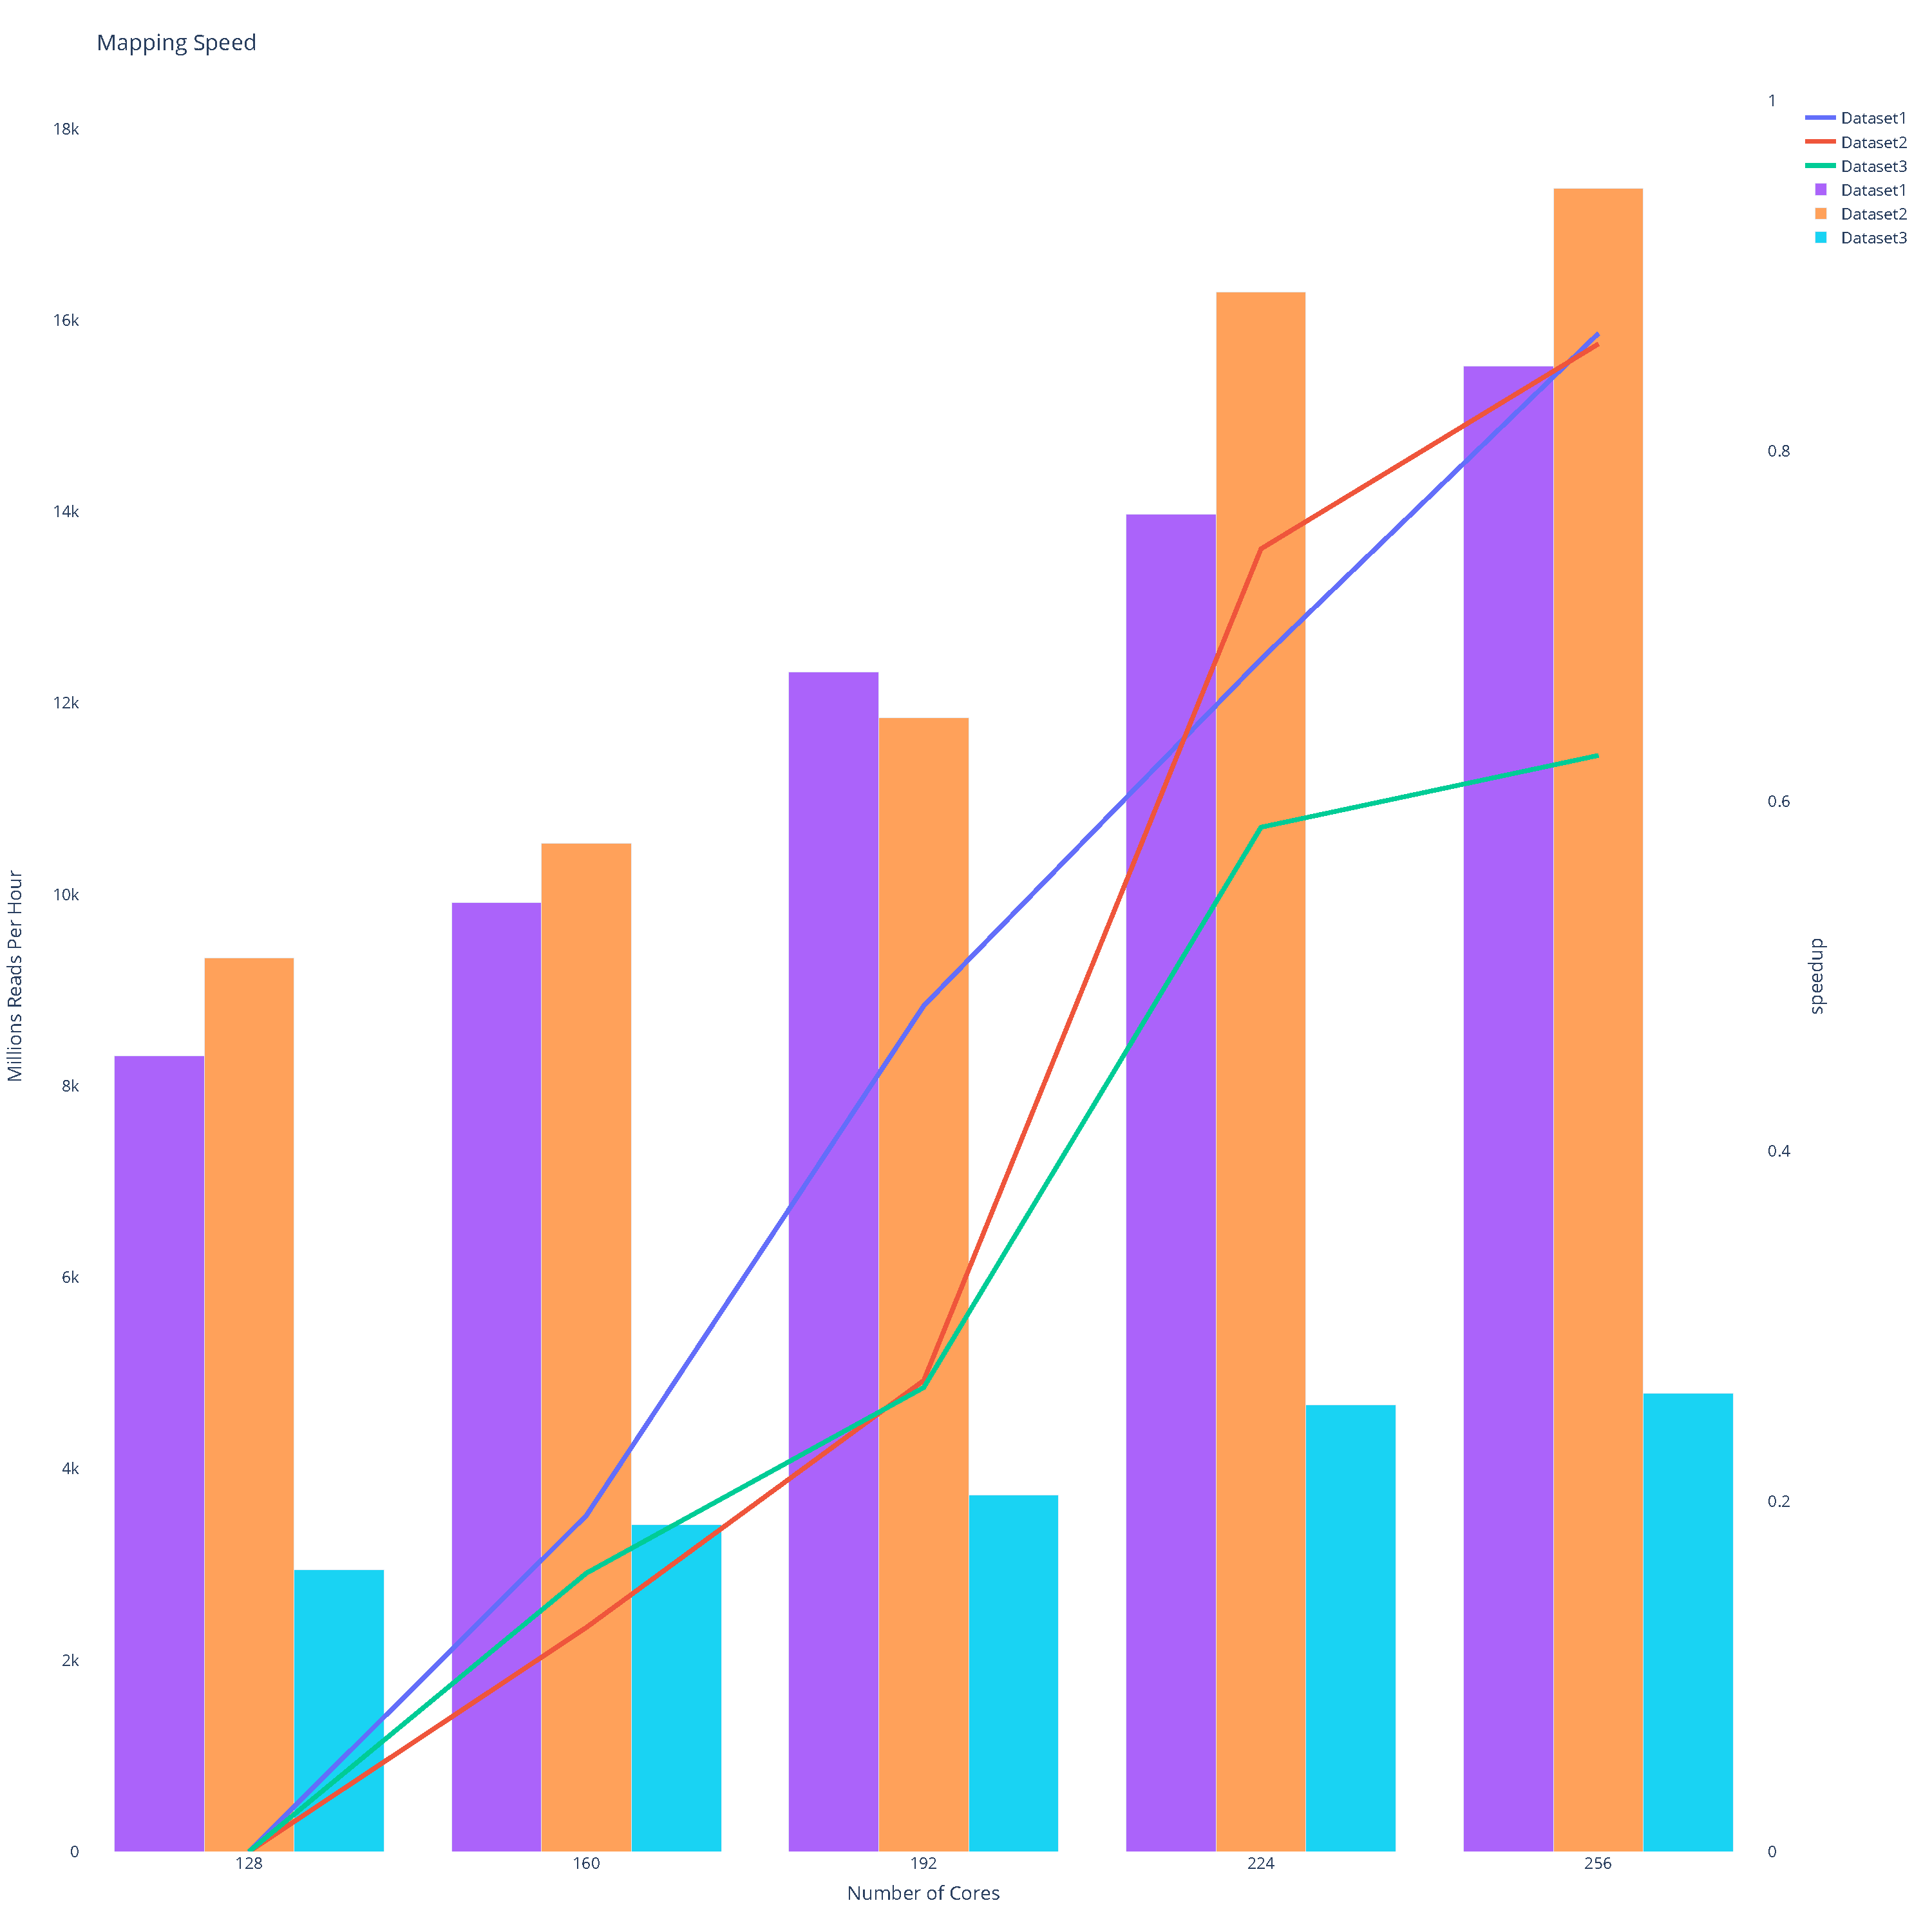
\includegraphics[width=0.5\textwidth]{Fig6.pdf}
	\caption{correlation of scSpark and UMI-tools.} \label{fig6}
  \end{figure}
As Fig~\ref{fig6} shown, we found scSpark's mapping speed achieved about 79\% parallel efficiency when CPU cores number increase from 128 to 256.
ScSpark enable distributed process align step per node across Spark cluster, so it can get nearly linear parallel efficiency.
So scSpark's align step is more scalability than tradition pipelines' aligner. 

\subsection{Biological verification} 
As Fig~\ref{fig9} shown, for each after processing cell barcode, their gene expression matrix approximate fit $y=x$, $R^{2}$ closed to 0.9998. 
\begin{figure}
  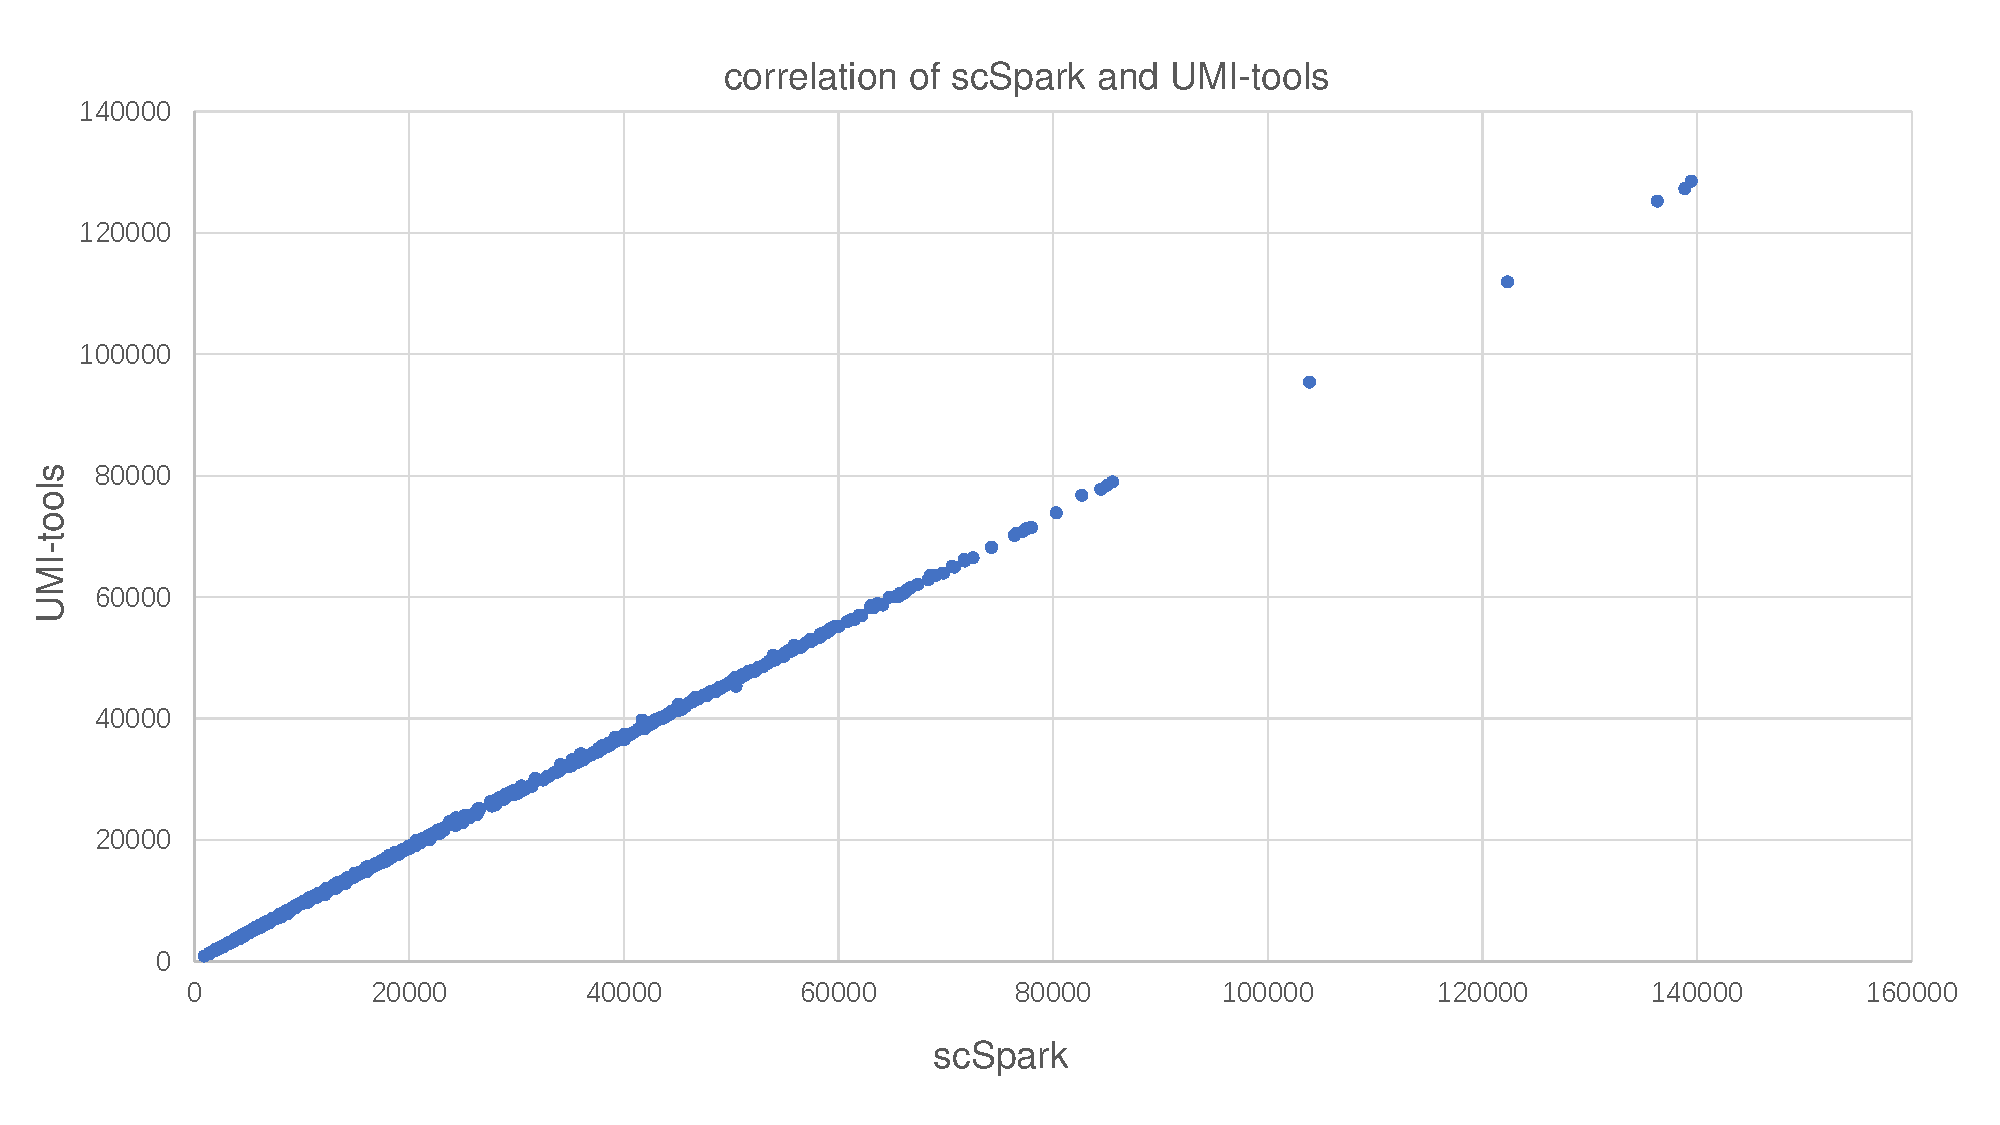
\includegraphics[width=0.5\textwidth]{fig9.pdf}
  \caption{correlation of scSpark and UMI-tools.} \label{fig9}
\end{figure}
Furthermore, we used Seurat to print tSNE picture which based on gene expression matrix generated by ScSpark and UMI-tools. 
And as Fig~\ref{fig10} shown, tSNE cell clustering result showed high corrleation between ScSpark and UMI-tools. 
\begin{figure*}
  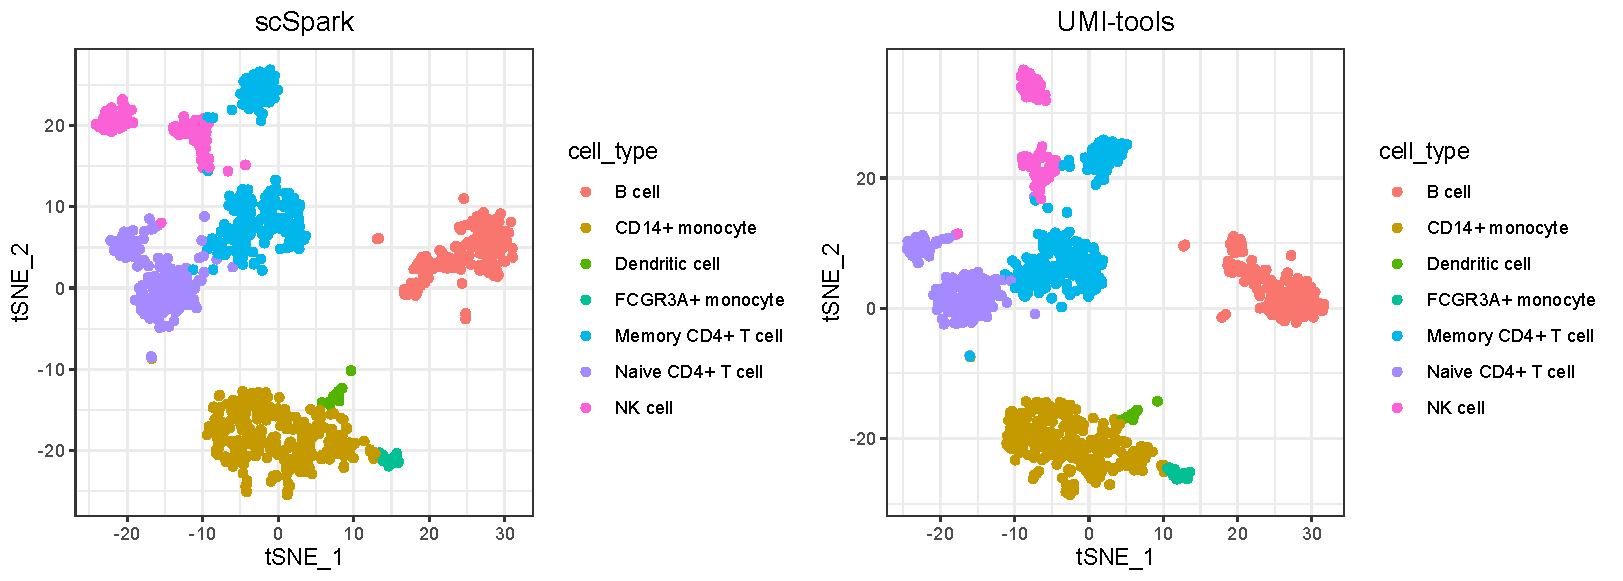
\includegraphics[width=\textwidth]{fig10.pdf}
  \caption{tSNE picture based on scSpark and UMI-tools' gene expression matrix.} \label{fig10}
\end{figure*}

\section{Conclusion}
In this paper, we proposed a way which utilize Apache Spark's in memory compute and distributed compute trait to strengthen upstream scRNA-seq pipeline.
We developed scSpark, which processes more efficiency and more scalable than tradition pipelines.

Refer to UMI-tools, scSpark divided the upstream process into four steps, UMI and CB correct, sequence quality control, genome alignment and transcript counting.
we found scSpark's can get higher performance than three tradition pipelines.
And we found scSpark's each steps can get higher performance than UMI-tools.
We also compared scSpark's result with UMI-tools to verified scSpark's result correct.

\bibliographystyle{IEEEtran}
\bibliography{reference}

\end{document}
